\documentclass{article}
\usepackage{amsmath}
\usepackage[utf8]{inputenc}
\usepackage{float}
\usepackage{epsfig,graphicx}
\usepackage{xcolor,import}
\usepackage[german]{babel}
\usepackage{textcomp}
\usepackage{mathtools}

\begin{document}
\thispagestyle{empty}
			\begin{center}
			\Large{Fakultät für Physik}\\
			\end{center}
\begin{verbatim}


\end{verbatim}
							%Eintrag des Wintersemesters
			\begin{center}
			\textbf{\LARGE WINTERSEMESTER 2014/15}
			\end{center}
\begin{verbatim}


\end{verbatim}
			\begin{center}
			\textbf{\LARGE{Physikalisches Praktikum 1}}
			\end{center}
\begin{verbatim}




\end{verbatim}

			\begin{center}
			\textbf{\LARGE{PROTOKOLL}}
			\end{center}
			
\begin{verbatim}





\end{verbatim}

			\begin{flushleft}
			\textbf{\Large{Experiment (Nr., Titel):}}\\
							%Experiment Nr. und Titel statt den Punkten eintragen
			\LARGE{5. Gasthermometer, Adiabatenexponent (Rüchardt), Dampfdichte nach Viktor Meyer}	
			\end{flushleft}

\begin{verbatim}

\end{verbatim}	
							%Eintragen des Abgabedatums, oder des Erstelldatums des Protokolls
			\begin{flushleft}
			\textbf{\Large{Datum:}}\Large{ 14.11.2014}
			\end{flushleft}
			
\begin{verbatim}
\end{verbatim}
							%Namen der Protokollschreiber
		\begin{flushleft}
			\textbf{\Large{Namen:}} \Large{Veronika Bachleitner, Erik Grafendorfer}
			\end{flushleft}

\begin{verbatim}


\end{verbatim}
							%Kurstag und Gruppennummer, zb. Fr/5
			\begin{flushleft}
			\textbf{\Large{Kurstag/Gruppe:}} \Large{Fr/1}
			\end{flushleft}

\begin{verbatim}






\end{verbatim}
							%Name des Betreuers, das Praktikum betreute.
			\begin{flushleft}
			\LARGE{\textbf{Betreuer:}}	\Large{SETMAN}	
			\end{flushleft}
\newpage
\section{Allgemeine Grundlagen}
Das Ideale Gas ist ein Modell, bei dem nur Wechselwirkungen durch Stöße der Teilchen untereinander und mit den Wänden angenommen werden.
\textbf{Gleichung des Idealen Gases:}
\begin{equation}
\label{gasgleichung}
pV=nRT
\end{equation}
Experimentell sind Ideale Gase solche, für die in guter Näherung das\\ \textbf{Boyle-Mariotte'sche Gesetz:}
\begin{equation}
\label{boyle-mariotte}
pV=const
\end{equation}
und das \textbf{Gay-Lussac'sche Gesetz:}
\begin{equation}
\label{gay-lussac}
p(t_C)=p(0)(1+\gamma_p t_C)
\end{equation}
erfüllt sind. (Aus \textit{Wagner, Reischl, Steiner: Einführung in die Physik})\\
\\
Hier ist $n$ die Anzahl der Mole der vorliegenden Substanzmenge und weiters
\begin{flushleft}
\begin{tabular}{|l|l|}
\hline Druck & $[p]=Pa$\\
\hline Volumen & $[V]=m^3$\\
\hline Gaskonstante & $R=8.3143 J K^{-1} mol^{-1}$, $R=k_B N_A$\\
\hline Boltzmannkonstante & $k_B=1.3806488*10^{23}J/K$\\
\hline Avogadro'sche oder &\\
Loschmidt'sche Zahl & $N_A=6.02214179*10^{23}$\\
\hline Absolute Temperatur & $[T]=^\circ C$\\
\hline
\end{tabular}
\end{flushleft}
\textbf{Definitionen\footnote{übernommen aus dem Anleitungstext}:}\\
\textbf{1 Mol} = Anzahl von Partikeln, die gleich groß ist wie die Anzahl der Atome in 12g des Isotops $^{12}C$, entspricht $N_A$. \\
\textbf{Molare Masse} = Masse eines Mols in g\\
\textbf{Molekularmasse} = Masse eines Moleküls, ausgedrückt in atomaren Masseneinheiten. \\
1 atomare Masseneinheit = $\frac{1}{12}$ eines $^{12}C$-Atoms.\\
1 amu = $\frac{1}{N_A}$=$1.6605 10^{-27}kg$\\
\textbf{Molekülmasse} = Masse eines Moleküls in g\\
\newpage
\section{Gasthermometer}
\subsection{Aufgabenstellung}
Wir zeigen die Gültigkeit des Boyle-Mariotte'schen Gesetzes (\ref{boyle-mariotte}) und bestimmen den Spannungskoeffizienten der Luft $\beta$ und die absolute Temperatur $T_0$ bei $0^\circ C$.\\
Dabei ermitteln wir auch den Zusammenhang zwischen Druck, Volumen und Temperatur der eingeschlossenen Luftmenge.
\subsection{Grundlagen}
\subsection{Versuchsaufbau und Methoden}
Wir halten die Temperatur konstant (Raumtemperatur) und ändern schrittweise h. Wir lesen dabei die zugehörigen Längen l der Luftsäule ab und multiplizieren diese mit den Gesamtdrücken p. 
$$pV=const \Rightarrow pl=const$$
\subsection{Ergebnisse}
Nachweis des Boyle-Mariotte'schen Gesetzes:\\

$$p_{\vartheta}=p_0 (1+\beta \vartheta)$$
$$\beta=\frac{1}{p_0}\frac{\Delta p}{\Delta \vartheta}=\frac{p_{\vartheta}-p_0}{p_0(\vartheta - \vartheta_0)}$$
$$T_0=$$
\\
Theoretischer Wert für ideale Gase:\\
$$\beta=\frac{1}{T_0}=\frac{1}{273.15K}$$

unsere p*V Werte
178953
17814.8
179628
178318
177024
177830
177328

Atmosphärischer Druck: $P_a=994.5mbar$\\
\\
Messung von l~V, h~$\Delta p$
\begin{center}
\begin{tabular}{r|l|l}
l in mm & h in mmHg & $\Delta p$ in mbar\\
\hline
221 & 62 & 82.46\\
200 & 143 & 190.19\\
186 & 218 & 289.94\\
173 & 283 & 376.39\\
162 & 345 & 458.85\\
154 & 407 & 541.31\\
139 & 528 & 702.24\\
\end{tabular}
\end{center}
Um zu zeigen, dass unsere Werte der Boyle-Mariotte Bedingung genügen, also ihr Produkt konstant ist, haben wir dieses Produkt für jedes Paar berechnet und mit seinem jeweils eigenen Unsicherheitsbereich geplottet. Dabei wird ersichtlich, dass wir durch alle Bereiche eine Gerade legen können - also liegen die Werte der Konstanten in ihren jeweiligen Vertrauensbereichen! Boyle-Mariotte gilt!
\begin{center}
\begin{figure}
\caption{Demonstration der Gültigkeit von Boyle-Mariotte, mit Gerade zur Anschaulichkeit}
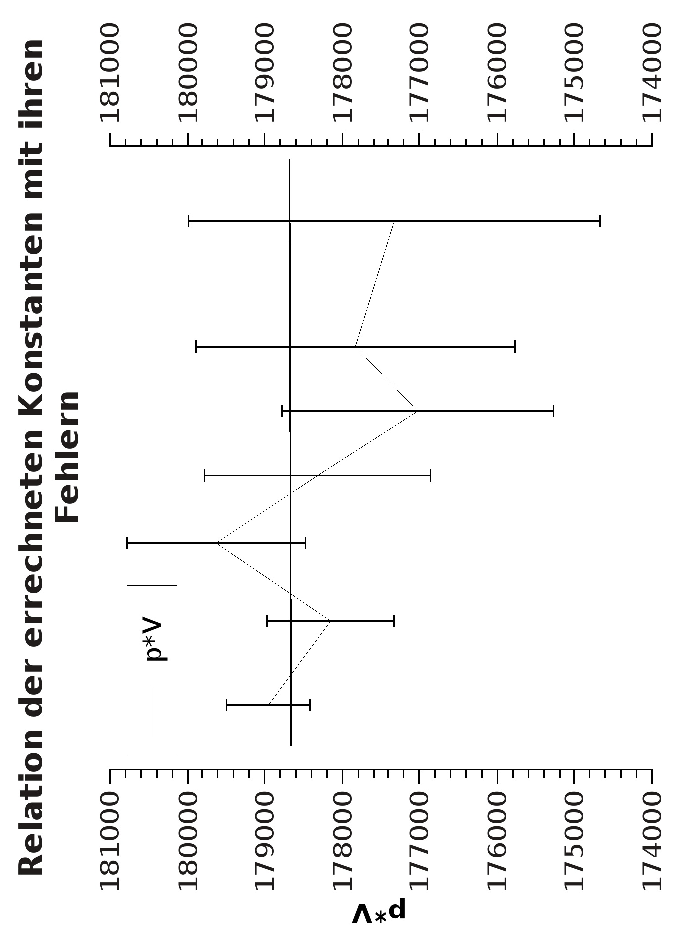
\includegraphics[scale=0.7, angle=-90]{konstanten.eps}
\end{figure}
\end{center}
2.
\subsection{Diskussion}

\newpage
\section{Bestimmung des Adiabatenexponenten der Luft nach Rüchardt}
\subsection{Aufgabenstellung}
Wir bestimmen den Adiabatenexponenten der Luft mit der Methode von Rüchardt.
\subsection{Grundlagen}
Der Adiabatenexponent ist die Hochzahl in folgender Gleichung:\\
$$p=const./V^{\kappa}$$
Er kann mit der Methode von Rückhardt bestimmt werden. Aus ihr folgt:
\begin{equation}
\label{kappa}
\kappa=(\frac{2\pi}{T})^2 \frac{mV_0}{q^2p}
\end{equation}
$$p=p_0+\frac{mg}{q}$$
\subsection{Versuchsaufbau und Methoden}
\subsection{Durchführung}
\subsection{Ergebnisse}
Wir machen 15 Messungen zu je 4 Schwingungen. Der Mittelwert der Messungen ist:\\
$$\bar{T}=1.09s$$
Masse der Kugel. (gemessen mit der Sartorius-Feinwaage ED2245)\\
$$m=16.700\pm0.005g$$

Der Standardabweichung des Mittelwerts unserer Messserie ist größer als die innere Messunsicherheit unserer Stoppuhr, also verwenden wir sie als unsere Unsicherheit $\Delta T$.
$$\Delta T=0.02s$$
Wir  berechnen $\kappa$ laut \ref{kappa}. \\
Mittels der Gaußschen Fehlerfortpflanzung erhalten wir $\Delta\kappa$:
$$\Delta\kappa=0.0505798$$
Also:
$$\boxed{\kappa=(1.375093 \pm 0.0505798)} $$

\subsection{Diskussion}
Wir verwenden die in der Aufgabenstellung angegebene Unsicherheit von $\pm$0.005g für die Masse der Kugel, obwohl die Waage eine Genauigkeit von $\pm$0.0003g erlauben würde. Aber es ist durchaus denkbar, nachdem wir eine nur eine Kopie der verwendeten Kugel gewogen haben, dass diese größere Unsicherheit gerechtfertigt ist. \\ 
Aufgrund eines peinlichen Fehlers bei einem Zaunpfostenproblem (dem Abzählen der Schwingungen an ihren Umkehrpunkten) haben wir nie 5 Schwingungen gemessen, sondern 4. Wir glauben aber, vor allem im Hinblick auf die Genauigkeit unseres Ergebnisses, dass wir diese Messungen verwenden können. \\ 
Wir würden für ein 2-Atomiges Molekül, nachdem es einen Freiheitsgrad f von 6 besitzt, ein $\kappa$ von $\frac{f+2}{f}=\frac{8}{6}\approx1.333333$ erwarten. Dieser erwartete Wert liegt im Vertrauensbereich des $\kappa$, das wir aus unseren Messungen berechnen. Wir sind stolz.
\newpage
\section{Dampfdichtebestimmung nach Viktor Meyer}
\subsection{Aufgabenstellung}
Wir bestimmen die Dampfdichte $\alpha$ und die Molekularmasse M einer Probesubstanz. 
\subsection{Grundlagen}
\textbf{Dampfdichte}: 
\begin{equation}
\label{dampfdichte_norm}
\alpha=\frac{\rho_{Gas}}{\rho_{L,N}}
\end{equation}
bei Normalbedingungen ($0^\circ C$, 1.01325 bar), wobei $\rho_{Gas}$ die Dichte des Gases, $\rho_{L,N}$ die Dichte der Luft bei Normalbedingungen.\\
\\
Umrechnung für ideale Gase, falls $T\neq 0$:
\begin{equation}
\frac{V_Dp}{T}=\frac{V_Np_N}{T_N}
\end{equation}
wobei $V_D$, $p$, $T$ bei Messbedingungen, $V_N$, $p_N$, $T_N$ bei Normalbedingungen.\\
\\
\textbf{Relative Dampfdichte:}
\begin{equation}
\label{dampfdichte_rel}
\alpha=\frac{\rho_N}{\rho_{L,N}}=\frac{\rho_D}{\rho_{L,N}}\frac{p_NT}{pT_N}
\end{equation}

\subsection{Versuchsaufbau und Methoden}
\subsection{Durchführung}
\subsection{Ergebnisse}

Masse des Kölbchens mit Halterung ohne Flüssigkeit: 7.4899g\\
Dichte der Luft bei Normalbedingungen ($0^\circ C$, 1.01325 bar):\\
$\rho_{L,N}=1.2931kg/m^3$

Setzen wir in (\ref{dampfdichte_rel}) ein, erhalten wir für die Dampfdichte:\\
%\alpha=\frac{\rho_N}{\rho_{L,N}}=\frac{\rho_D}{\rho_{L,N}}\frac{p_NT}{pT_N}\\
\\
Daraus die Molekularmasse:\\
$$M_{Gas}=\alpha*M_L=\alpha*28.98$$

\subsection{Diskussion}
\end{document}
